% Chapter Template

\chapter{Results} % Main chapter title

\label{Results} % Change X to a consecutive number; for referencing this chapter elsewhere, use \ref{ChapterX}

\lhead{4. \emph{Results}} % Change X to a consecutive number; this is for the header on each page - perhaps a shortened title

%----------------------------------------------------------------------------------------
%	SECTION 1
%----------------------------------------------------------------------------------------
 We consider a model with 5 sequences ($N=5$) and 30 columns ($M=30$), with magic words of length 10 ($W= 10 $). 
 
 \section{Convergence}
 We first want to estimate the number of iterations that are necessary for the Markov chain to converge to the target distribution. We run the sampler for 200 iterations, with $\alpha' = (1, 1,1,1)$ and $\alpha = (12,7,3,1)$ and obtain the results in figure \ref{fig:1}. We can see that the burn-in period is almost undetectable and the chain converges rapidly. Nonetheless, to estimate the accuracy, we discard the first $100$ samples and save the subsequent samples with a lag of $10$. We obtain an accuracy of $80\%$ : the true starting positions being $[11, 11, 18, 5, 4]$ and the estimated positions being $[11, 12, 18, 5, 4]$. We can also note that for the second sequence, the estimated start position 12 is close to the true start position 11, and inside the magic word.
 \begin{figure}[htbp]
  \centering
    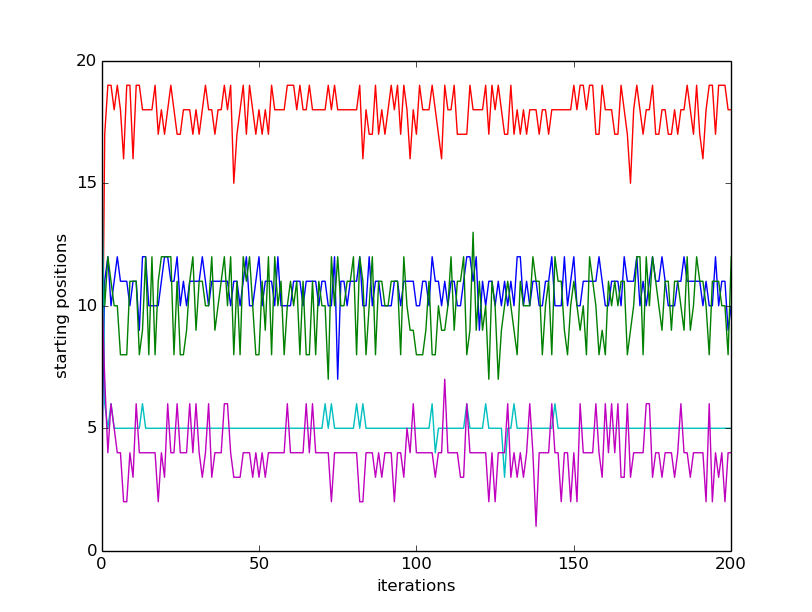
\includegraphics[scale = 0.75]{Figures/fig1}
  \caption{Markov chain samples for $\alpha' = (1, 1,1,1)$ and $\alpha = (12,7,3,1)$}
  \label{fig:1}
\end{figure}

Another way to check the convergence of the Markov Chain is to estimate how far the samples are from perfect mixing. We can therefore compute the R.hat (potential scale reduction factor). For that, we run 3 chains, compute the variance of the samples from each chain (after the halves of each have been discarded. We also compute the variance of all the chains mixed together. 
\begin{equation*}
R.hat = \sqrt{\frac{\text{mixture variance}}{\text{average within the chain variances}}}
\end{equation*}
After 200 iterations of the chain described above, we obtain : $R.hat = 1.02$, which indicates that the chain has converged, since the distributions between and within the chains are identical.

\section{Effect of $\alpha$}

The accuracy of the estimation depends on whether the categorical distributions of the magic words and of the background are distinguishable. It would therefore follow that the more skewed $\alpha$ is, or the more different from $\alpha'$, the higher the accuracy will be.

Since the accuracy can be highly dependent on the sequences we generated, we compute the average accuracy for $500$ sets of sequences, for different vectors $\alpha$. The results are presented in table \ref{alpha}

\begin{table}[h]
\centering
\caption{Accuracy for different values of $\alpha$. model with $\alpha' = (1, 1,1,1)$}
\label{alpha}
\begin{tabular}{|l|l|}
\hline
$\alpha$              & Accuracy \\ \hline
$(12, 7, 3, 1)$       & 0.61        \\ \hline
$(12, 7, 20, 16)$     & 0.63       \\ \hline
$(2, 2, 2, 2)$        & 0.402       \\ \hline
$(12, 1, 1, 1)$ & 0.74       \\ \hline
\end{tabular}
\end{table}

The lowest accuracy is for $\alpha = (2, 2, 2, 2)$ as expected, since it is very close to the prior for the background. Wee can see the accuracy the highest when the Dirichlet parameter is “tilted” towards one of the letters $\alpha = (12, 1, 1, 1)$. The difference between the components of $\alpha$ and $alpha'$ seems to have less impact on the accuracy than the skewness of $Dir(\alpha)$.
Figure \ref{fig:2} shows the convergence plot for a set of sequences using $\alpha' = (1, 1,1,1)$ and $\alpha = (12, 1, 1, 1)$. The accuracy for this data set is $80\%$: the true positions are $[1,9,17,5,11]$ and the estimated positions are $[1,9,17,5, 10]$.  

 \begin{figure}[htbp]
  \centering
    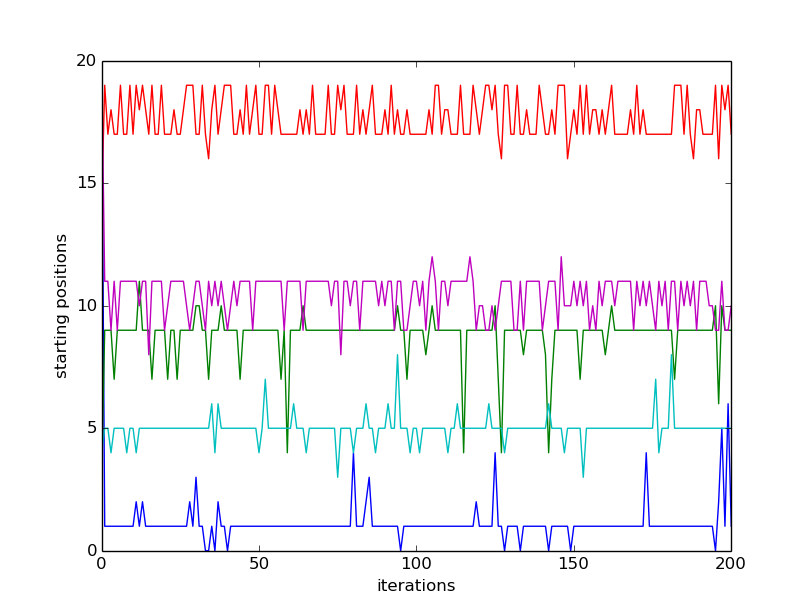
\includegraphics[scale = 0.75]{Figures/fig2}
  \caption{Markov chain samples for $\alpha' = (1, 1,1,1)$ and $\alpha = (12, 1, 1, 1)$}
  \label{fig:2}
\end{figure}

\section{Effect of the lag}
We have considered that the estimated starting position is the mode of the posterior distribution $p(r_n | R_{-n}, D)$. It seems reasonable to think that the less correlated the samples we draw (after convergence) are, the more accurate our estimation of the node will be. To verify this, we compute the average accuracy for $500$ sets of sequences, for different values of the lag. To get a better estimation of the mode, we run the Gibbs sampler for $500$ iterations but only discard the first $100$ samples, since we have seen that the convergence is achieved rapidly. The results are presented in table \ref{lag}

\begin{table}[h]
\centering
\caption{Accuracy for different lag lengths, model with $\alpha' = (1, 1,1,1)$ and $\alpha = (12,7,3,1)$}
\label{lag}
\begin{tabular}{|l|l|}
\hline
Lag        & Accuracy \\ \hline
1 (no lag) &     0.66    \\ \hline
10 samples &     0.67    \\ \hline
30 samples &     0.63    \\ \hline
\end{tabular}
\end{table}
 
As we can see, the difference between no lag and a lag of 10 samples is not significant, and with a lag of 30 samples, the average accuracy is even slightly lower. we conclude that the purpose of saving every $k$th iteration for our application is not statistical, since the correlation doesn't seem to influence the accuracy. However, it could have computational benefits if we run multiple chains with a very high number of samples in parallel and do not want to carry them all around in our simulation.
 